\section{Week 02}

\subsection{27/07/2015}

\textbf{Stage and copy file from CERN servers}

Patrick have copied all the .slcio files in his directory and processed them with Marlin using two bash scripts. We have copied the ntuples from eos (see the glossary) to our folder, and now we can loop among them. 

He used two files: jobCopy.sh and jobMarlin.sh to process the files.

jobCopy first stage the files from the tape (Castor) to the disk, and then copies the files into EOS folder.
jobMarlin loops above all the files writing the correct steering.xml file and create all the ntuple.

\textbf{More about the slcio ntuples}

We have found out something else about our ntuples: 

We discovered that all the top quark have status 3, and the bottoms have sometimes status 2 and sometimes status 3.

By using the parent information (mcpa0 e mcpa1, for daughters mcda0,1,2,3,4) we managed to select only the leptons which come from the W decay. Then, with a pyroot macro we filled the 2-D histograms of the number of leptons versus the energy and the angle.


\subsection{28/07/2015}

\textbf{Lepton vs energy-angle histogram}

We managed to loop above all the .root files. We use 256 bins (16 for the angle and 16 for the energy), that are quite similar to the square root of the entries (they are about 40k, the 40\% of 100k events).\\
We have also used the reduced energy defined as \[x=\frac{2E}{m_t} \sqrt{\frac{1-\beta}{1+\beta}} \]   \[ \beta =\sqrt{1-4m_t^2/s} \]
We plotted the histo of the number of lepton in function of the $cos(\theta)$ and of the reduced energy. We expected a curve distribution in both the variables, and, to do this, we have to plot only the positive leptons (or the negative); otherwise there can't be any asymmetry in the angular distribution.

The result can be seen in figure \ref{02_Electrons}, \ref{02_Muons}, \ref{02_Electrons+muons}

\begin{figure} [ht!]
  \centering
  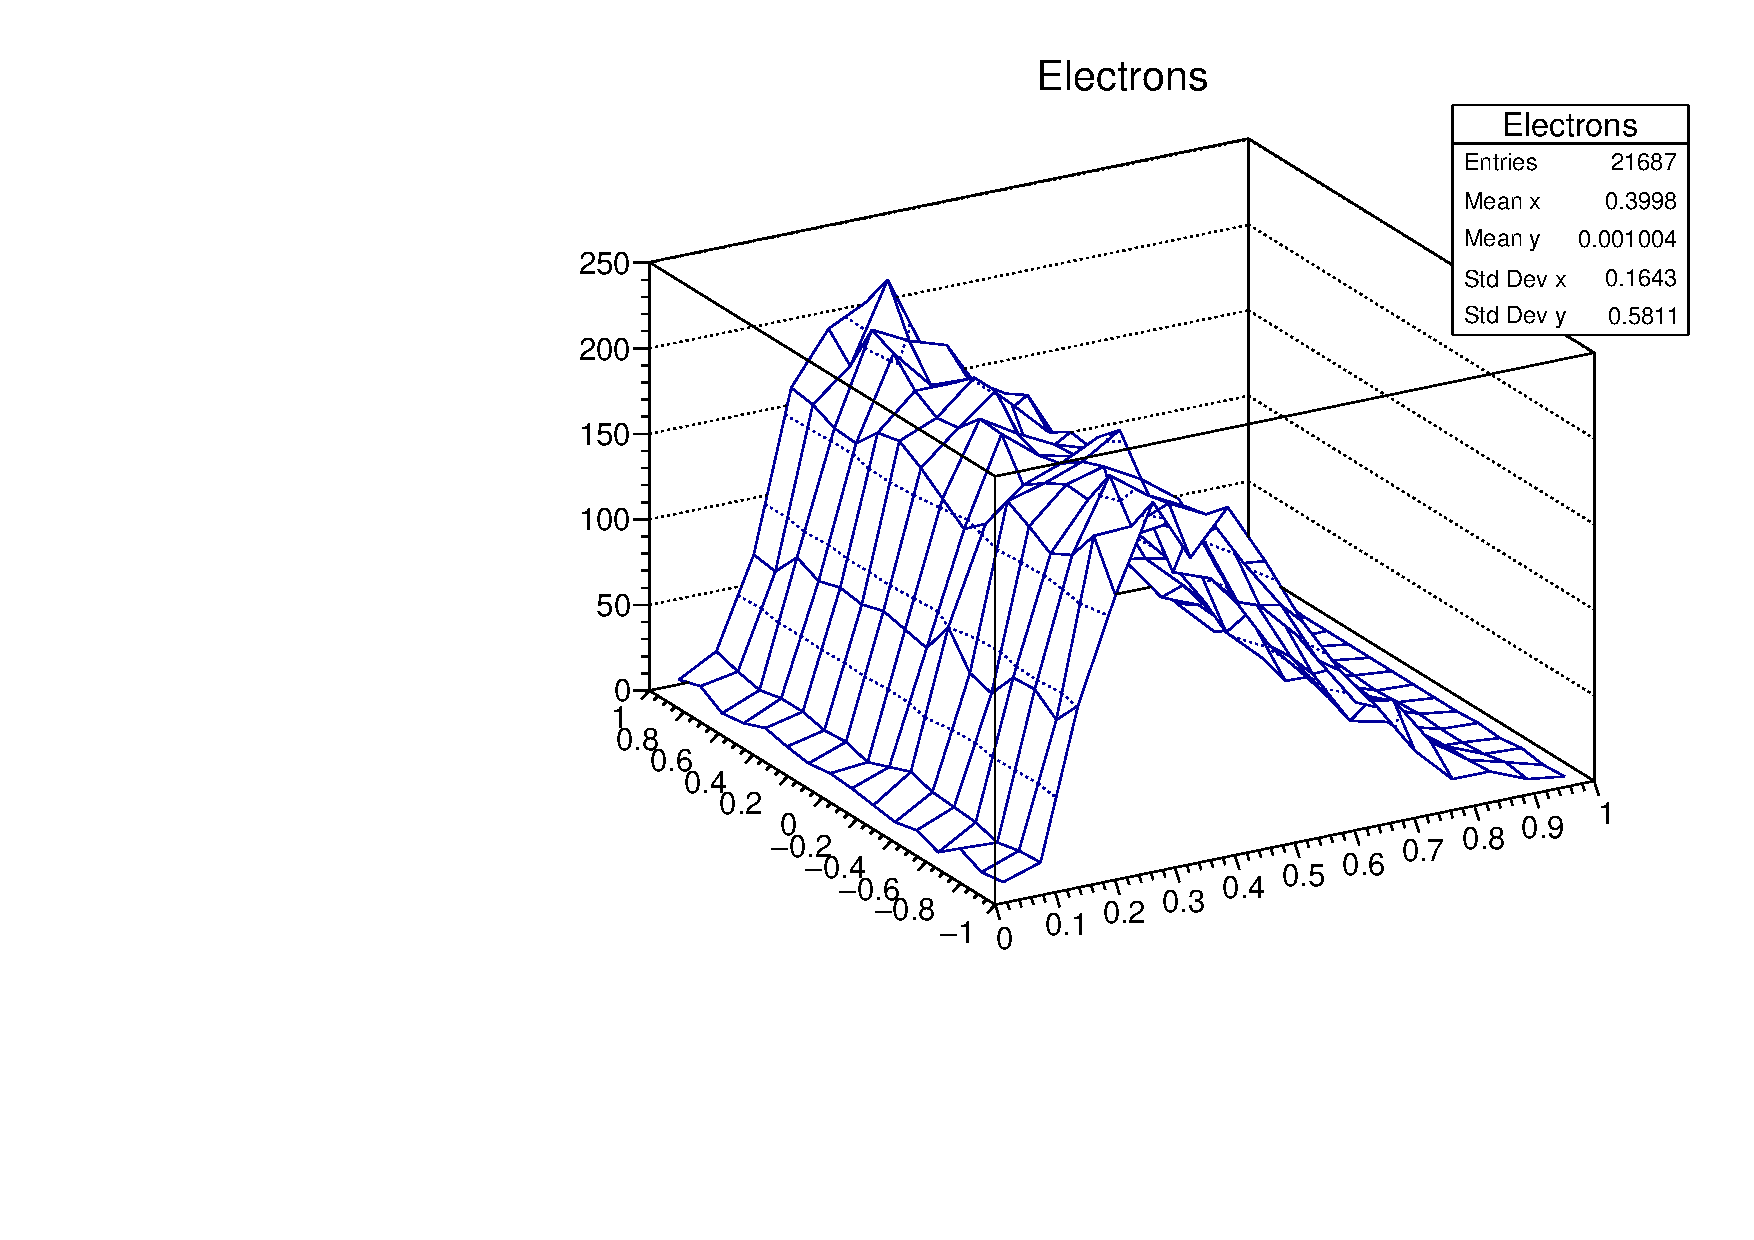
\includegraphics[width=0.7\textwidth]{02_Electrons.pdf}
 \caption{Energy-angle distribution of the electrons}
 \label{02_Electrons}
\end{figure}

\begin{figure} [ht!]
  \centering
  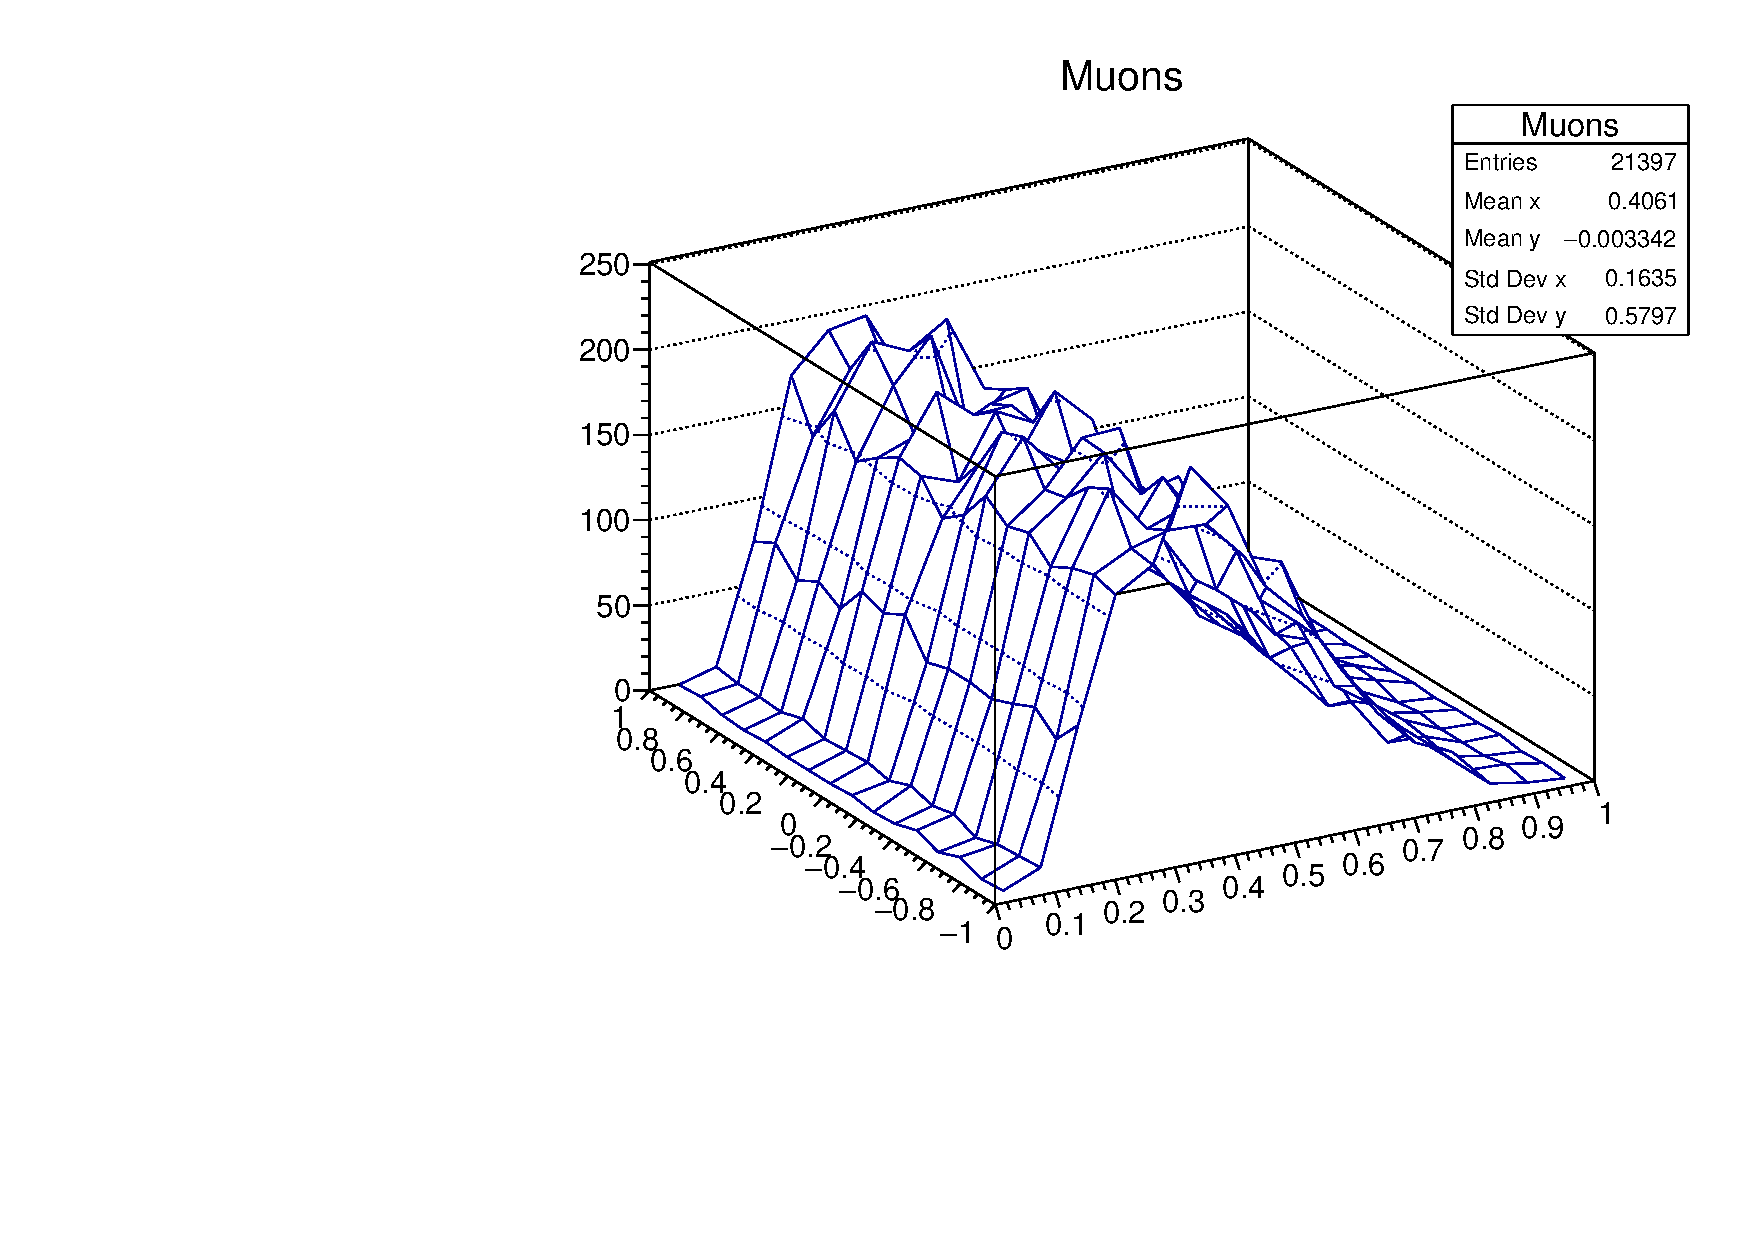
\includegraphics[width=0.7\textwidth]{02_Muons.pdf}
 \caption{Energy-angle distribution of the negative muons}
 \label{02_Muons}
\end{figure}

\begin{figure} [ht!]
  \centering
  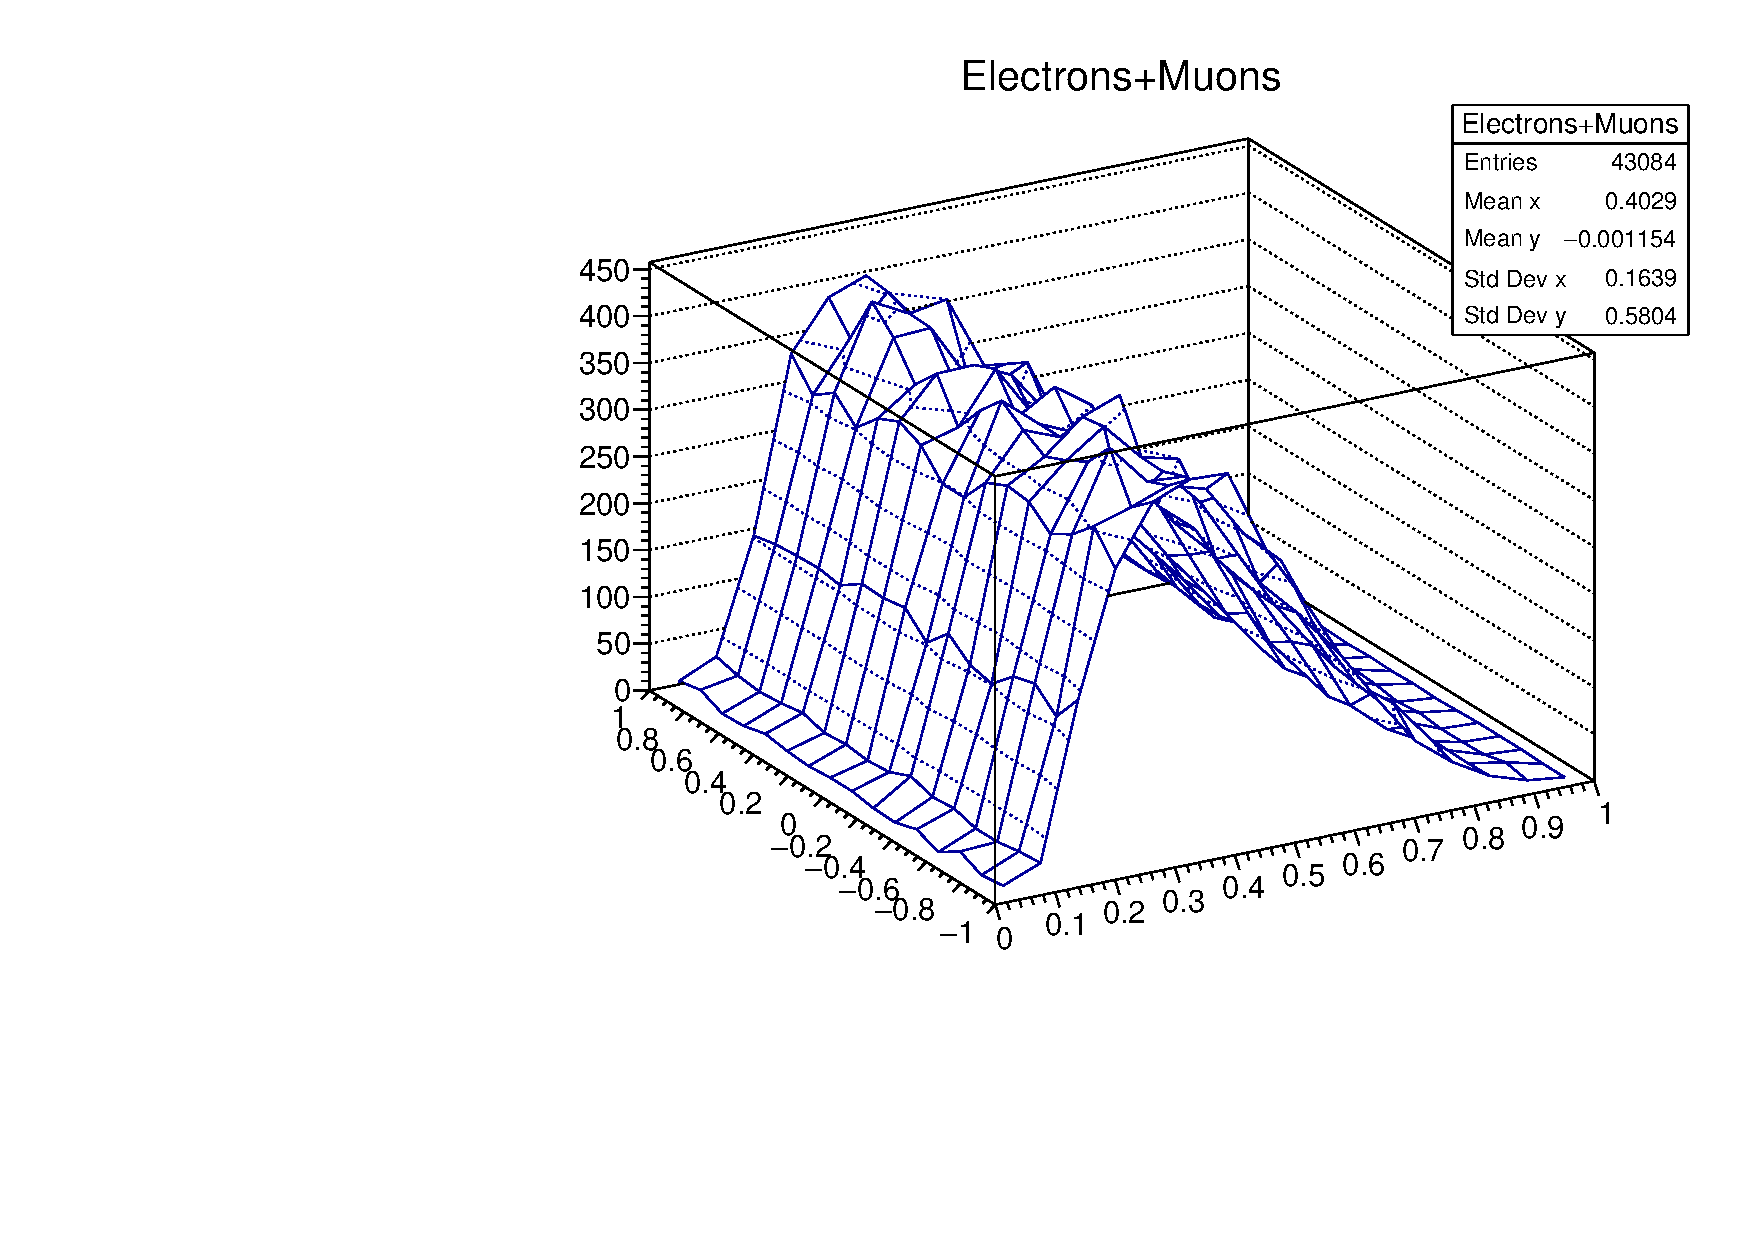
\includegraphics[width=0.7\textwidth]{02_Electrons+muons.pdf}
 \caption{Energy-angle distribution of the electrons and negative muons}
 \label{02_Electrons+muons}
\end{figure}

Unfortunately the angular distribution is flat: this implies that Pythia simulation don't consider the top polarization. So we cannot use these simulation to perform our analysis, and we need to proceed with different data.

\textbf{Writing Root Tree using PyROOT}

We have also learn how to write a Tree Root using PyROOT. We need first to define a TTree variable, then define the branches, and then fill the branches with a 0-D array (this is important), by looping on the events.
Further information in the glossary folder.

\subsection{29/07/2015}

\textbf{Copy and Marlin new simulation files}

We decided to use other simulation files made with Wizard (instead that Pythia), we could find them at this site \href{https://twiki.cern.ch/twiki/bin/view/CLIC/MonteCarloSamplesForTopPhysics?sortcol=2;table=3;up=1#sorted_table.}{clicca qui}
These simulations are made at 365 GeV and would consider the polarization of the top quarks (we hope so).

By using some scripts bash we have staged all the files, copied and Marlin them.

\subsection{30/07/2015}

\textbf{Whizard ntuples}

We have started to analyze the new ntuples obtained with Whizard simulation. The tree branches have the same name. Though we found out that all the events contains the following particles:
0,1 : the two incoming electrons
2,3 : the two incoming electrons after radiating soft photons
4,5 : the two soft photons
6,7,8,9,10,11 : the final state of the event with b an $\bar{b}$ quark, a couple quark and anti-quark, the electron (positron) we are looking for with index 10 and the correspondent neutrino.

So we have simply plotted the distribution of the electron with index 10 and we found out that the angular distribution has the asymmetry we are looking for.\\
Now we are going to run our script on lxplus looping all the data.

In addition we discover that we have not always the resonant state in the simulation, and sometimes we have a top without an antitop (or viceversa); so we don't know very well how the simulation was made. We don't care to this fact very much for the moment. 

\subsection{31/07/2015}

\textbf{Whizard ntuples}

The result of the plot with all date is visible in figure \ref{02_Energy_angle_MC}.

\begin{figure} [ht!]
  \centering
  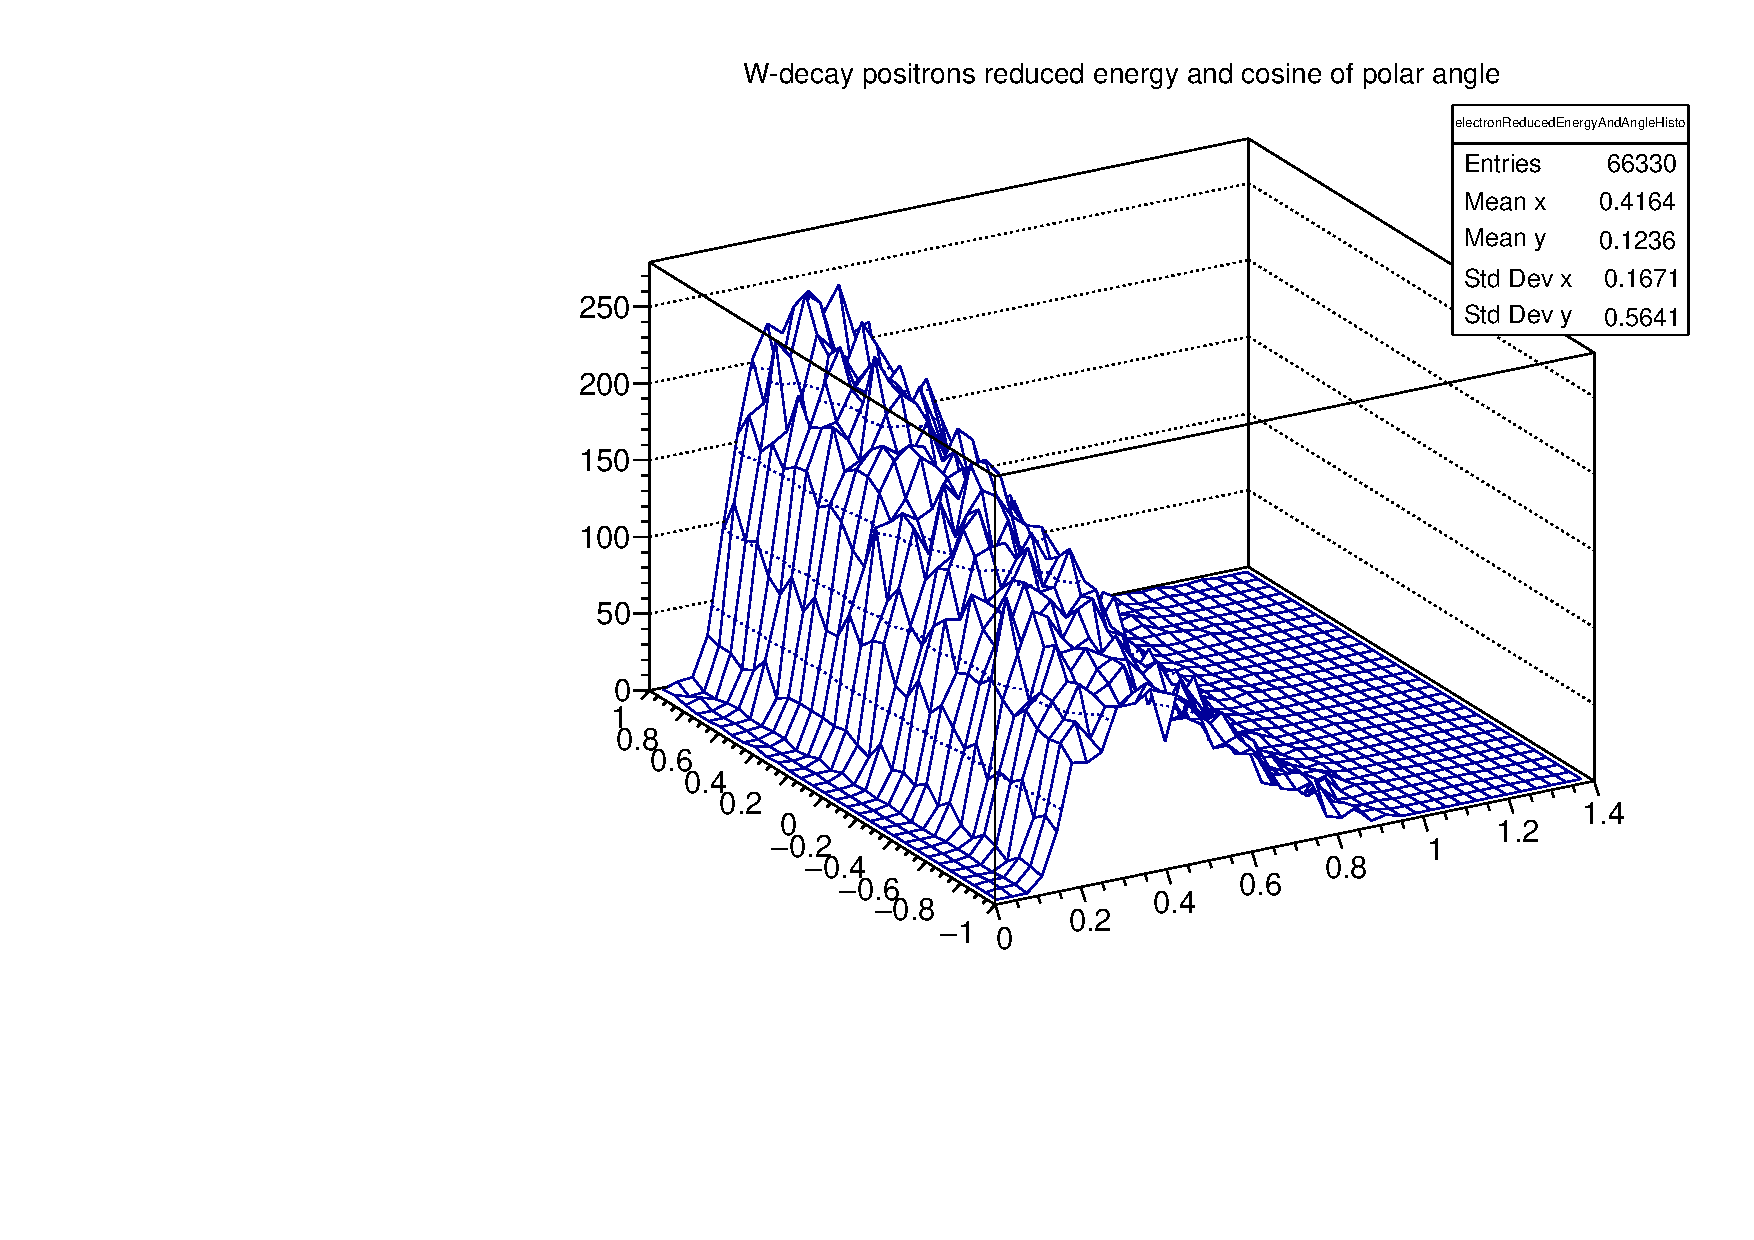
\includegraphics[width=0.7\textwidth]{02_Montecarlo_electron_distribution.pdf}
 \caption{Energy-angle distribution of the electrons simulated by Whizard}
 \label{02_Energy_angle_MC}
\end{figure}

We have then compared this distribution with the one calculated analytically (figure \ref{02_Energy_angle_AN}), and, by making the ratio of the two histograms we obtained something really flat (figure \ref{02_Energy_angle_ratio}), so the two distributions agree. There are some spike in the ratio of the two histograms near the boundary of the allowed energy. This is due to the fact that probably the top mass and the W mass were chosen approximately (we found out that the top mass were chosen to be 174 GeV), and the maximum energy of the electrons depends a lot on the top mass.

\begin{figure} [ht!]
  \centering
  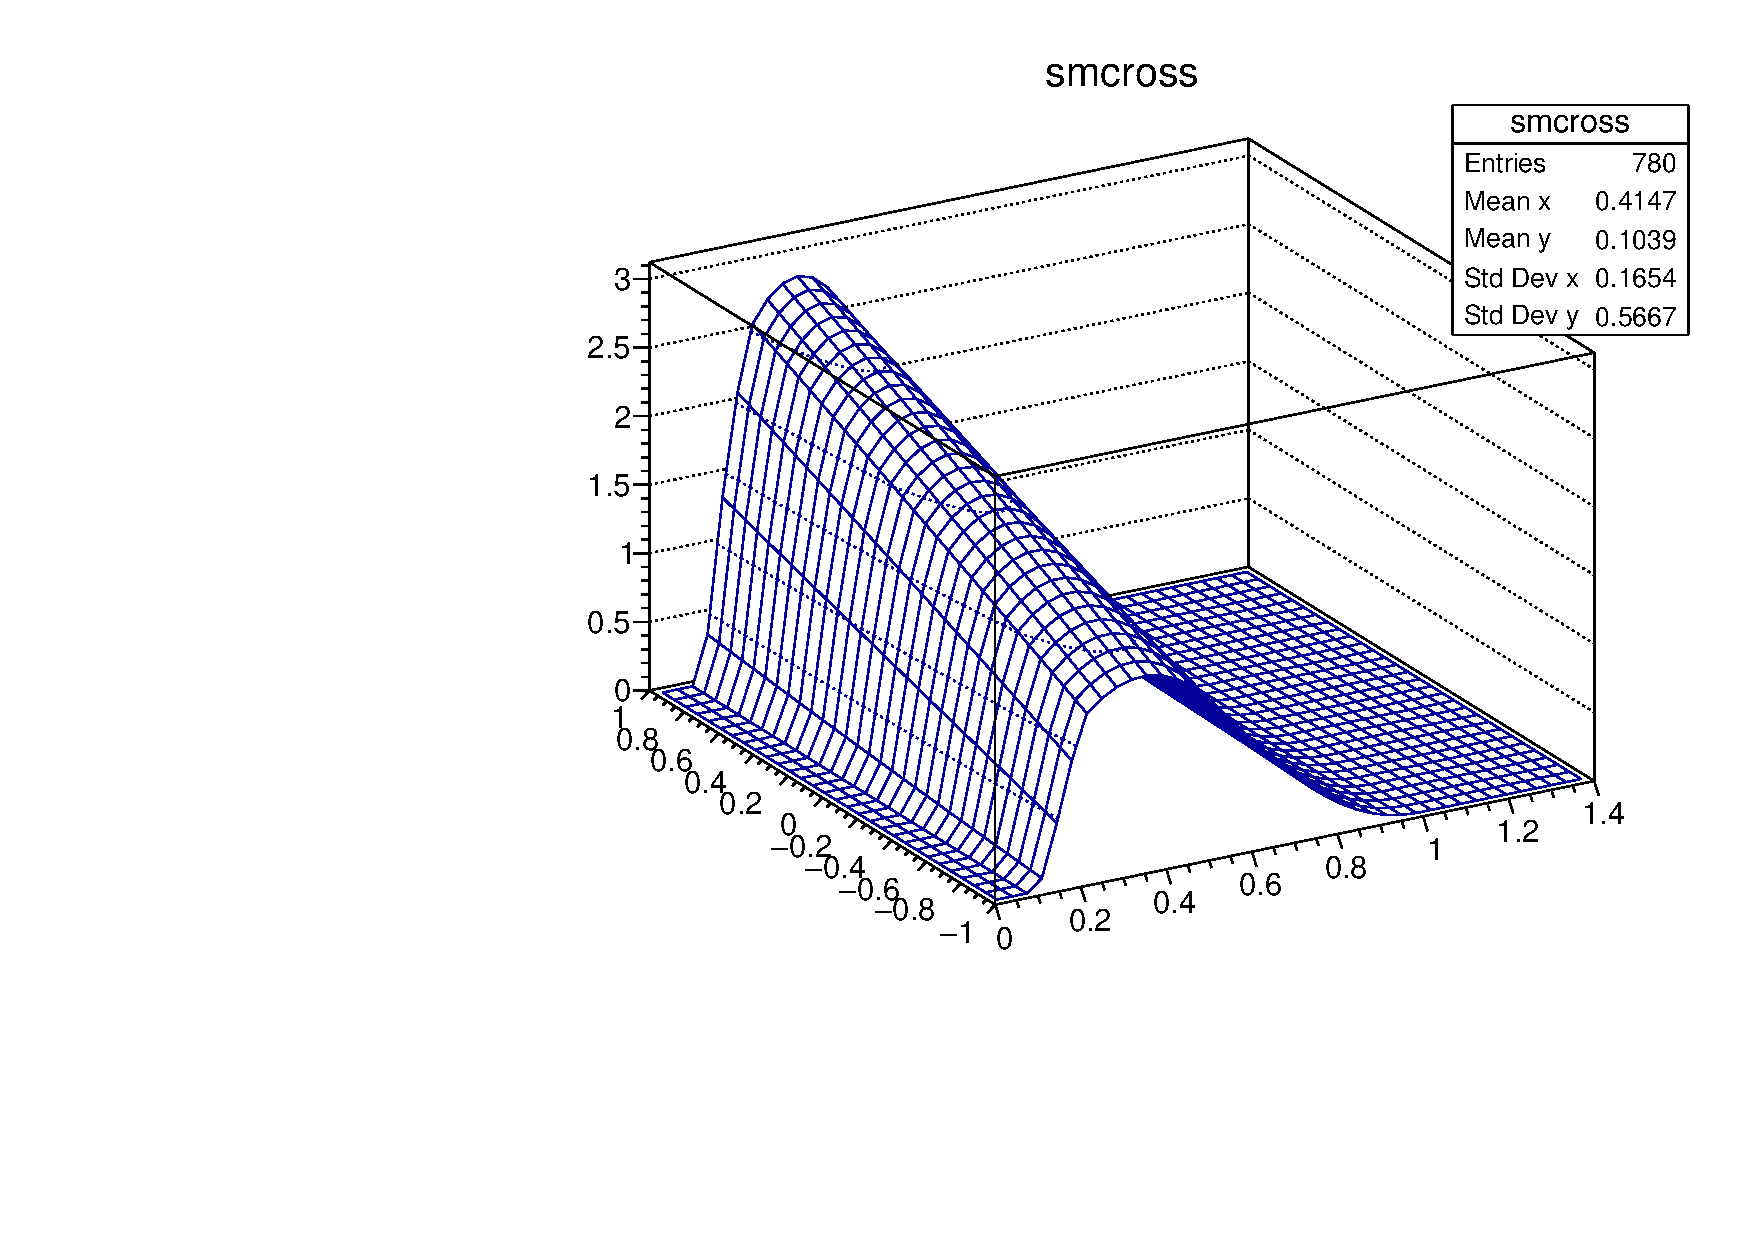
\includegraphics[width=0.7\textwidth]{02_Analytic_electron__distribution.pdf}
 \caption{Energy-angle distribution of the electrons calculated analytically}
 \label{02_Energy_angle_AN}
\end{figure}

\begin{figure} [ht!]
  \centering
  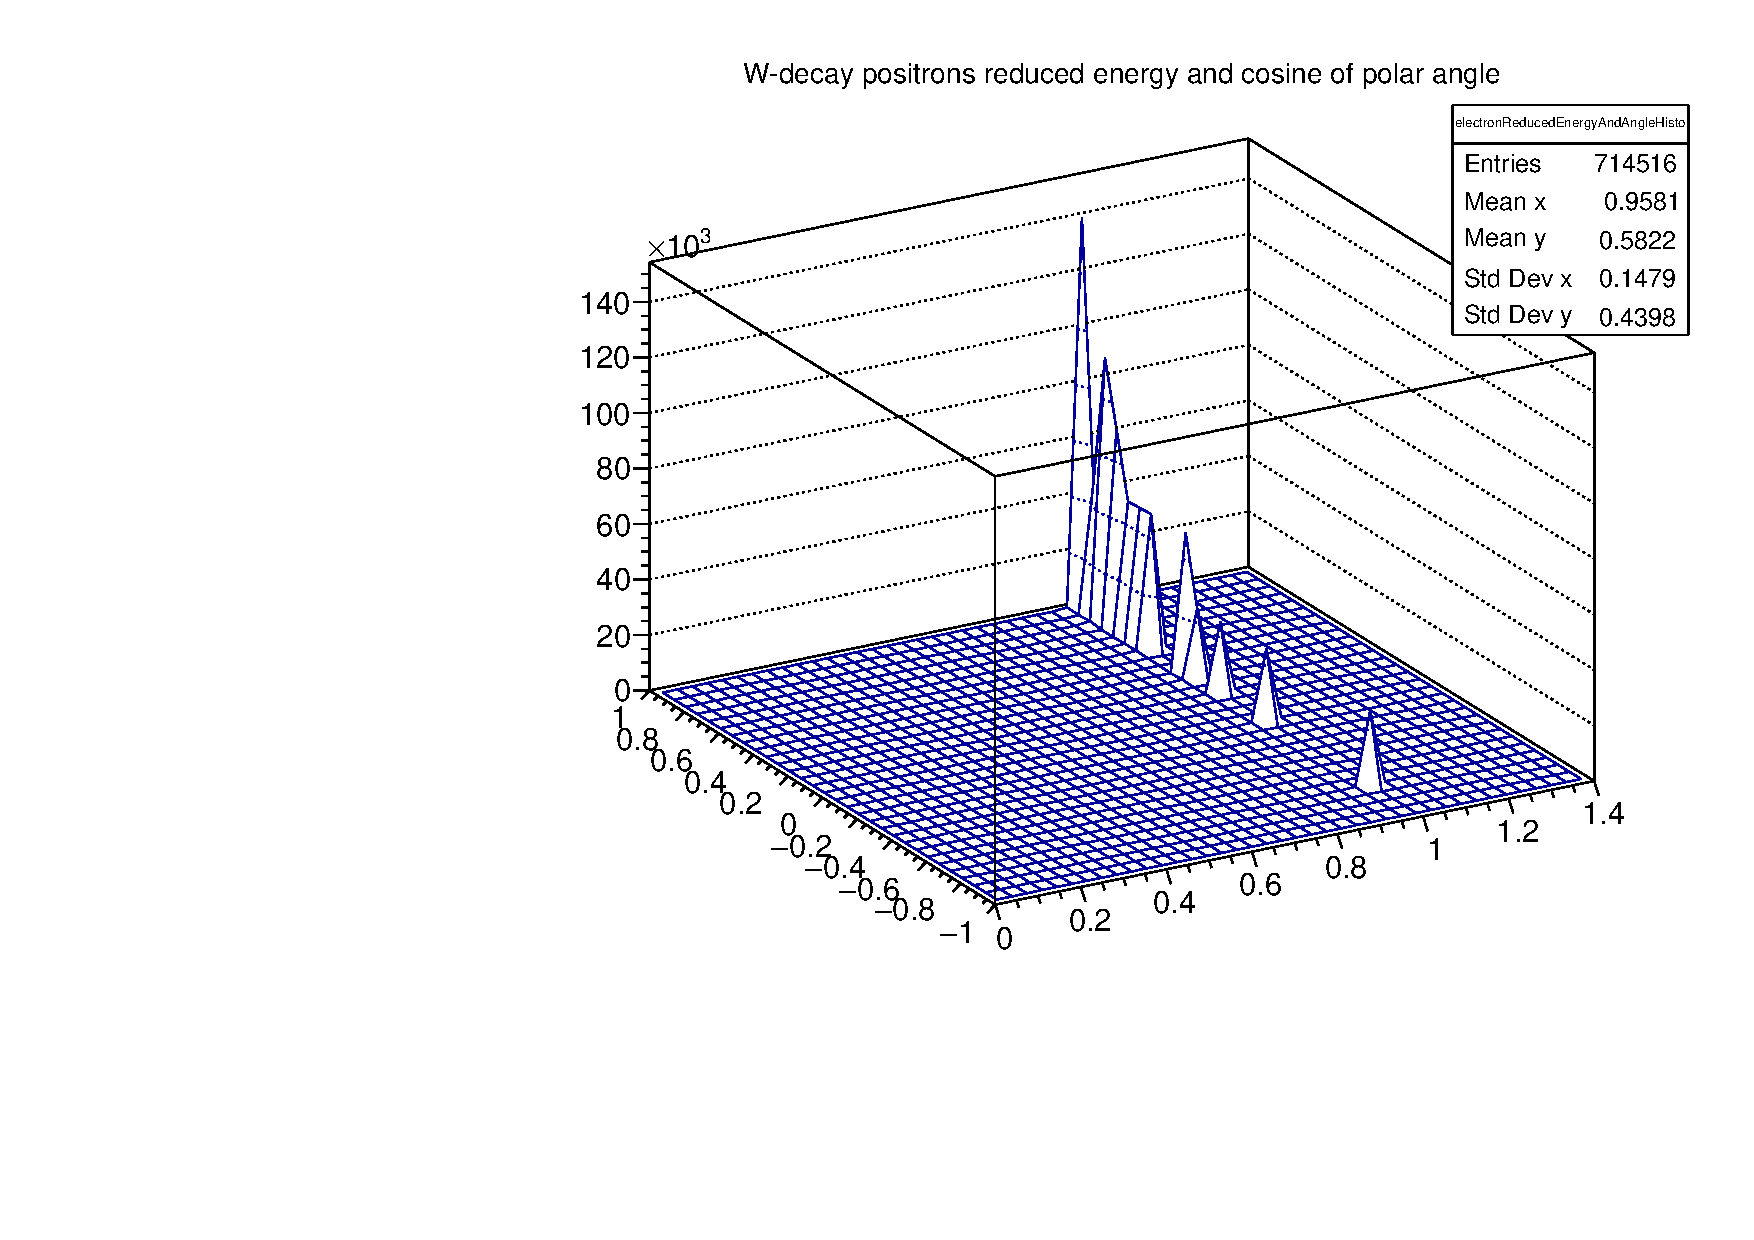
\includegraphics[width=0.7\textwidth]{02_Ratio_MC_An.pdf}
 \caption{Ratio of the distribution simulated and analytic}
 \label{02_Energy_angle_ratio}
\end{figure}

If we better analyze the ratio by zooming on the distribution in the flat region, we can see that there are many fluctuations that are due to the little quantity of data. 

\begin{figure} [ht!]
  \centering
  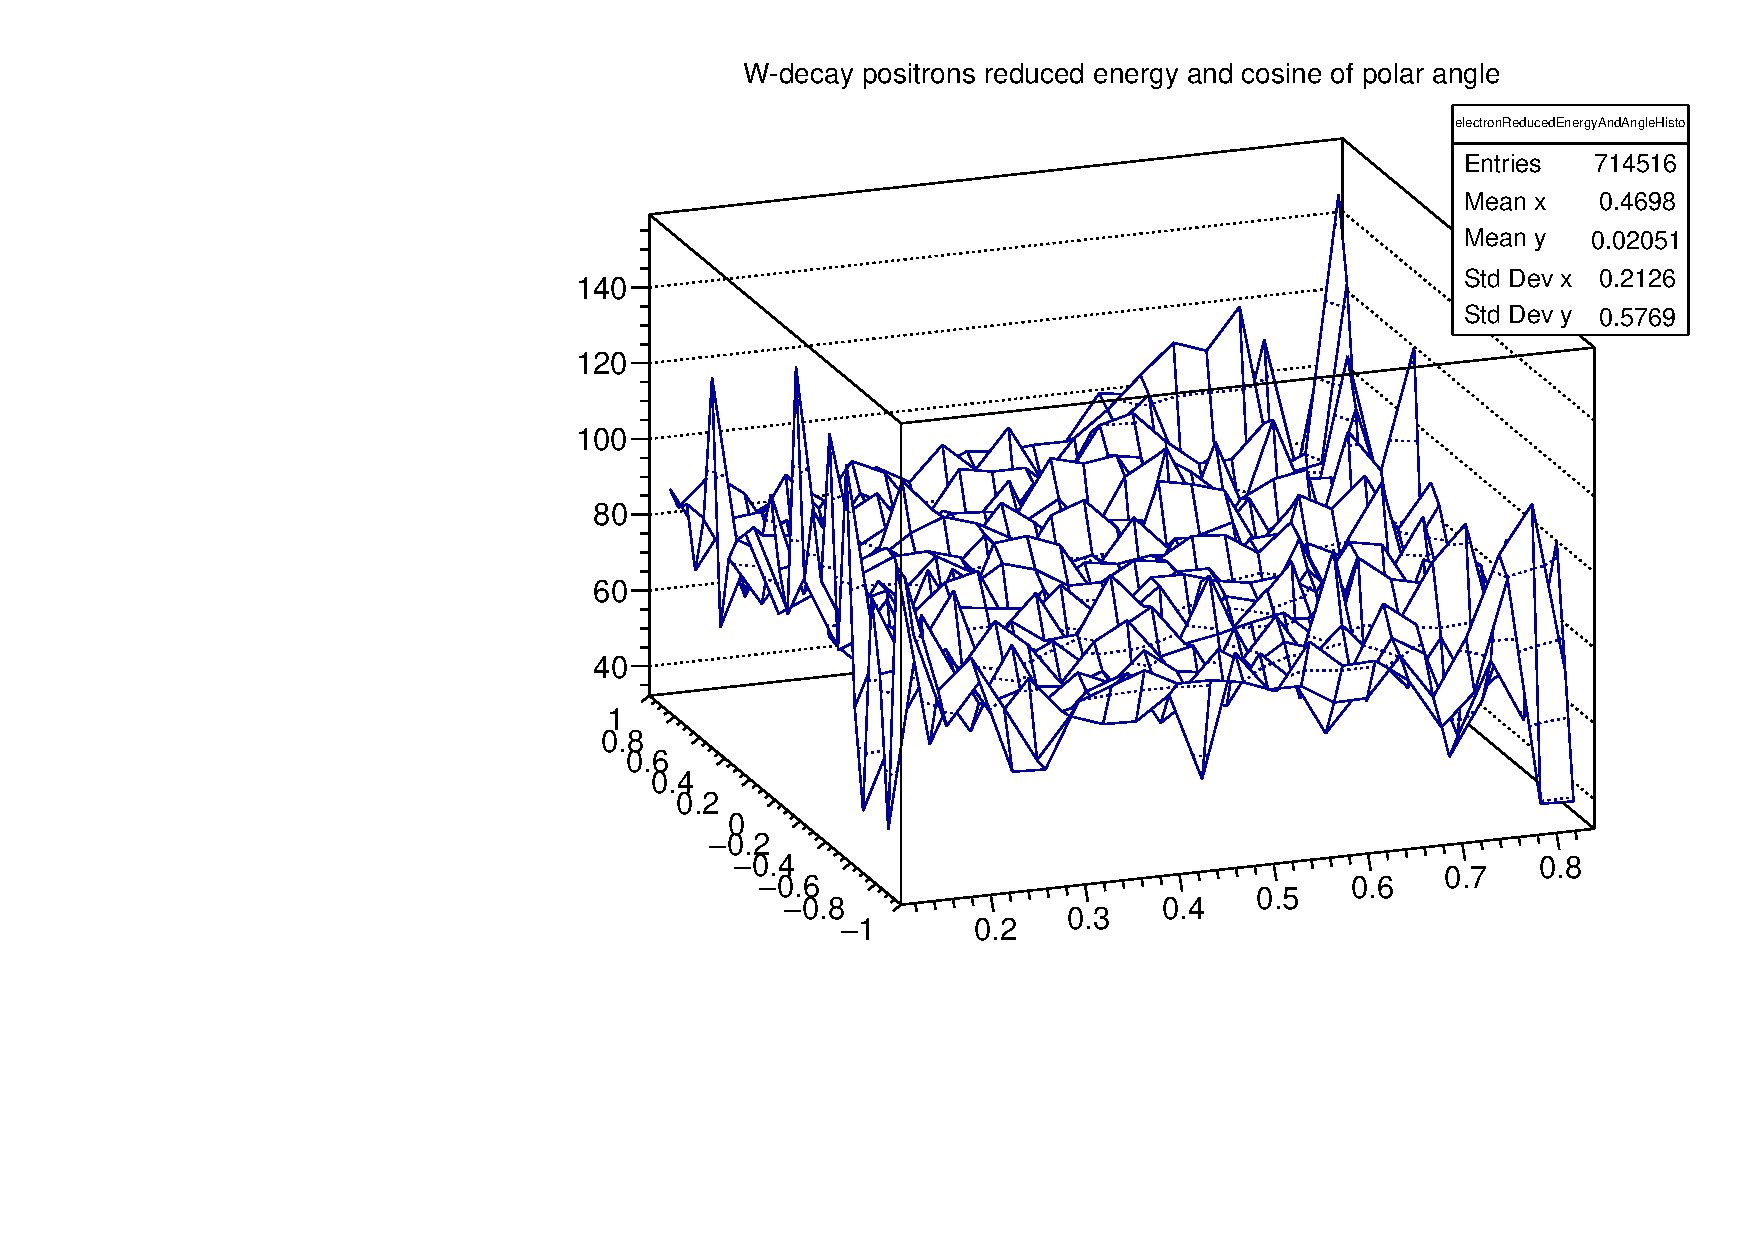
\includegraphics[width=0.7\textwidth]{02_Ratio_MC_An_zoom.pdf}
 \caption{Zoom of the ratio of the distribution simulated and analytic}
 \label{02_Energy_angle_ratio_zoom}
\end{figure}

In the end we can say that our work can start, because our data take in account the polarization effect.

\subsection{Other leptons simulations}

We have just started to stage, copy and Marlin also the files containing one muon or tau.